\documentclass{beamer}[10]
\usepackage{pgf}
\usepackage{beamerthemesplit}
\usepackage[utf8]{inputenc}
\definecolor{kugreen}{RGB}{151,209,251}
\definecolor{kugreenlys}{RGB}{50,158,139}
\definecolor{kugreenlyslys}{RGB}{173,190,177}
\definecolor{kugreenlyslyslys}{RGB}{214,223,216}
\setbeamercovered{transparent}
\mode<presentation>
\usetheme[numbers,totalnumber,compress,sidebarshades]{PaloAlto}
\setbeamertemplate{footline}[frame number]
 
  \usecolortheme[named=kugreen]{structure}
  \useinnertheme{circles}
  \usefonttheme[onlymath]{serif}
  \setbeamercovered{transparent}
  \setbeamertemplate{blocks}[rounded][shadow=true]
 
\logo{\includegraphics[width=1.6cm]{HHU_Logo.pdf}}
\title{Algorithmus zur Berechnung der metrischen Dimension eines Kaktusgraphen}
\author{Alina Elterman}
\institute{Lehrstuhl f\"ur Algorithmen und Datenstrukturen\\ Heinrich-Heine-Universit\"at}
\date{\today}  
\begin{document}

\frame{\titlepage} 

%\frame{\frametitle{Inhaltsverzeichnis}
%\tableofcontents
%} 



\section{Kaktusgraph} 
\frame{\frametitle{Definition: Kaktusgraph}
\begin{itemize}
\item{Definition:\\ 
Ein Graph ist ein Kaktusgraph genau dann, wenn alle einfachen Kreise paarweise kantendisjunkt sind. (Teilen sich höchstens einen gemeinsamen Knoten.)}
\end{itemize}}
%\frame{\frametitle{Manipulation und Bestechung}
%\begin{itemize}
%\item {Bei Manipulation und Bestechung werden die Bewertung der W\"ahler \"uber die Kandidaten ge\"andert. \\
%\begin{itemize}
%\item Manipulation: W\"ahler sind vorgegeben!\\
%\item Bestechung:  W\"ahler werden frei ausgesucht!
%\end{itemize}}
%\end{itemize} 
%}
\frame{\frametitle{Eigenschaften von Kaktusgraphen}
\begin{itemize}
\item Zweifache Zusammenhangskomponenten sind:
\begin{itemize}
\item Kreise
\item einzelne Kanten
\end{itemize}
\item Beispiele: Bäume, Wege, Kreise, Freundschaftsgraphen, Sonnen und Halbsonnen
\item Außenplanar
\item Anzahl Kanten:\\ 
$|E|$ = Anzahl Knoten $|V|$ + Anzahl Kreise $|C|$ -1\\mit $|C|\leq \frac{|V|}{2}$ 
(Man braucht mind. 2 (kreisfreie) Knoten um einen neuen Kreis zu bilden)
\end{itemize}
}

\section{Algorithmus}

\subsection{Beispiel} 
\frame{\frametitle{Beispiel}
\begin{table}[htb]
     \centering
\begin{tabular}{ccc}
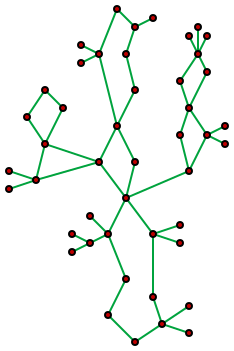
\includegraphics[width=120pt]{bilder/Cactus_graph.pdf}&$\;\;\;\;\;\;\;\;\;\;\;\;\;\;$&
\includegraphics[width=100pt]{bilder/alg1.pdf}
\end{tabular}
\end{table}
}

\frame{\frametitle{Beispiel}
\begin{table}[htb]
     \centering
\begin{tabular}{ccc}
\includegraphics[width=120pt]{bilder/Cactus_graph1.pdf}&$\;\;\;\;\;\;\;\;\;\;\;\;\;\;$&
\includegraphics[width=100pt]{bilder/alg2.pdf}
\end{tabular}
\end{table}
}

\frame{\frametitle{Beispiel}\begin{table}[htb]
     \centering
\begin{tabular}{ccc}
\includegraphics[width=120pt]{bilder/Cactus_graph2.pdf}&$\;\;\;\;\;\;\;\;\;\;\;\;\;\;$&
\includegraphics[width=100pt]{bilder/alg3.pdf}
\end{tabular}
\end{table}
}

\frame{\frametitle{Beispiel}\begin{table}[htb]
     \centering
\begin{tabular}{cc}
\includegraphics[width=180pt]{bilder/Cactus_graph3.pdf}&
\includegraphics[width=100pt]{bilder/alg4.pdf}
\end{tabular}
\end{table}
}

\frame{\frametitle{Beispiel}\begin{table}[htb]
     \centering
\begin{tabular}{cc}
\includegraphics[width=180pt]{bilder/Cactus_graph4.pdf}&
\includegraphics[width=100pt]{bilder/alg5.pdf}
\end{tabular}
\end{table}
}

\frame{\frametitle{Beispiel}\begin{table}[htb]
     \centering
\begin{tabular}{cc}
\includegraphics[width=180pt]{bilder/Cactus_graph5.pdf}&
\includegraphics[width=100pt]{bilder/alg6.pdf}
\end{tabular}
\end{table}}

\frame{\frametitle{Beispiel}\begin{table}[htb]
     \centering
\begin{tabular}{ccc}
\includegraphics[width=140pt]{bilder/Cactus_graph6.pdf}&$\;\;\;\;\;$&
\includegraphics[width=100pt]{bilder/alg7.pdf}
\end{tabular}
\end{table}}

\frame{
\frametitle{Beispiel}
\begin{table}[htb]
     \centering
\begin{tabular}{c|c}
\includegraphics[width=140pt]{bilder/Cactus_graph6.pdf}&
\includegraphics[width=120pt]{bilder/Cactus_graph7.pdf}
\end{tabular}
\end{table}
}



%%%%%%%%%%%%%%%%%%%%%%%%%%%%%%%%%%%%%%%%%%%%%%%%%%%%%%%%%%%%%%%%%%%%%%%%%%%%%%%%%%%%%%%%%%%%%%%%%%%%%%%%%%%%%%%%%%%%%%%%%%%%%

\section{Beweis} 

\subsection{Laufzeit} 
\frame{\frametitle{Laufzeit}
\includegraphics[width=300pt]{bilder/lz1.pdf}
}
\frame{\frametitle{Laufzeit}
\includegraphics[width=300pt]{bilder/lz2.pdf}
}
\frame{\frametitle{Laufzeit}
\includegraphics[width=300pt]{bilder/lz3.pdf}
}
\frame{\frametitle{Laufzeit}
\includegraphics[width=300pt]{bilder/lz4.pdf}
}
\frame{\frametitle{Laufzeit}
\includegraphics[width=300pt]{bilder/lz5.pdf}
}
\frame{\frametitle{Laufzeit}
\includegraphics[width=300pt]{bilder/lz6.pdf}
}
\frame{\frametitle{Laufzeit}
\includegraphics[width=300pt]{bilder/lz7.pdf}
}
\frame{\frametitle{Laufzeit}
\includegraphics[width=300pt]{bilder/lz8.pdf}
}
\subsection{AmalKnoten}
\frame{\frametitle{Finden}
\begin{itemize}
\item Knoten der Klasse $A$\pause
\item {Knoten in mindestens zwei ZSK?
\begin{itemize}
\item an zwei ZSK\pause
\item{ an einem ZSK und mit einem Weg?
\begin{itemize}
\item NEIN-Sonne/Halbsonne
\item JA, wenn noch etwas an dem Knoten ist!
\end{itemize}}
\item Knoten mit $deg >3$
\end{itemize}}
\pause
\item mindestens ZSK und Baum(ohne Weg dazwischen)
\item bei mehreren ZSK zählt Weg auch als Komponente
\item bei mehreren ZSK zählt Weg vom Baum(ohne Weg dazwischen) auch als Komponente
\end{itemize}
}
\frame{\frametitle{Erkennen}
\begin{itemize}
\item Während der Berechnung der MD von ZSK
\item Regeln 
\begin{itemize}
\item Nie an einer Sonne
\item Nie an einer ZSK mit einem Ankerknoten (Ausnahme: gerader Kreis)
\item usw. 
\end{itemize}
\end{itemize}
Im schlimmsten Fall muss geprüft werden ob der Abstand zu den 2(!) nächsten Ankerknoten $>\frac{n}{2}$ ist.
}


\frame{\frametitle{Vorkommen}
\includegraphics[width=200pt]{bilder/zskamal1.pdf}
~\newline
Lösung: Nimm von jedem Knoten Anzahl der Mengen -1 Knoten in die MB auf
}

\frame{\frametitle{Vorkommen}
\includegraphics[width=200pt]{bilder/zskamal2.pdf}
~\newline
Lösung: Setze Knoten in die MB aus der Menge mit max. Anzahl Amalknoten
}
\frame{\frametitle{Berechnung AmalKnoten}
\includegraphics[width=200pt]{bilder/amalknotenpresi1.pdf}
}
\frame{\frametitle{Berechnung AmalKnoten}
\includegraphics[width=200pt]{bilder/amalknotenpresi2.pdf}
}
\frame{\frametitle{Berechnung AmalKnoten}
\includegraphics[width=200pt]{bilder/amalknotenpresi3.pdf}
}

\frame{\frametitle{Berechnung AmalKnoten}
Idee: Schließe die unnützeste Komponente aus!\\
Beispiel 1: Weg
\newline\newline\newline
\includegraphics[width=100pt]{bilder/zskamal3.pdf}
}

\frame{\frametitle{Berechnung AmalKnoten}
Falls keine Wege vorhanden:\\
1. Finde alle Amalknoten mit einer Komponente mit Anzahl AmalKnoten $=1$ (Tiefensuche)\\
2. Initialisiere damit eine Liste von Amalknoten\\
3. Arbeite die Liste ab und aktualisiere sie.
}

\frame{\frametitle{Berechnung AmalKnoten}
\begin{itemize}
\item Jeder Knoten kommt maximal einmal rein und wird maximal einmal abgearbeitet.
\item Jede Komponente wird einmalig entfernt (Der Algorithmus läuft einmal durch sie durch und aktualisiert alle Amalknoten (-1). )
\item Falls ein Amalknoten verschwindet, aktualisiere Anzahl der Amalknoten an den Komponenten (1, oder 0) 
Um zu prüfen teste ob der AmalKnoten in der Liste war.
\end{itemize}
Bemerkung: Es gibt immer eine Komponente mit einem Amalknoten (sonst gäbe es einen nicht einfachen Kreis!)
}
\frame{\frametitle{Berechnung AmalKnoten}
\vspace{+4mm}
\includegraphics[width=300pt]{bilder/zskamal4.pdf}

}
\subsection{Korrektheit} 
\frame{\frametitle{Korrektheit}
Probleme sind äquivalent:\\Einen Kaktusgraphen zu Trennen $\Longleftrightarrow$ Alle Komponenten und die Nachbarschaften von AmalKnoten zu Trennen.
%\includegraphics[width=280pt]{pd3.jpeg}
}
\frame{\frametitle{Korrektheit}
Ein Teilgraph welcher durch das Entfernen eines Knotens entsteht ist entweder ein Weg oder hat mindestens ein Element der metrischen Basis.
}
\frame{\frametitle{Korrektheit}
\centering
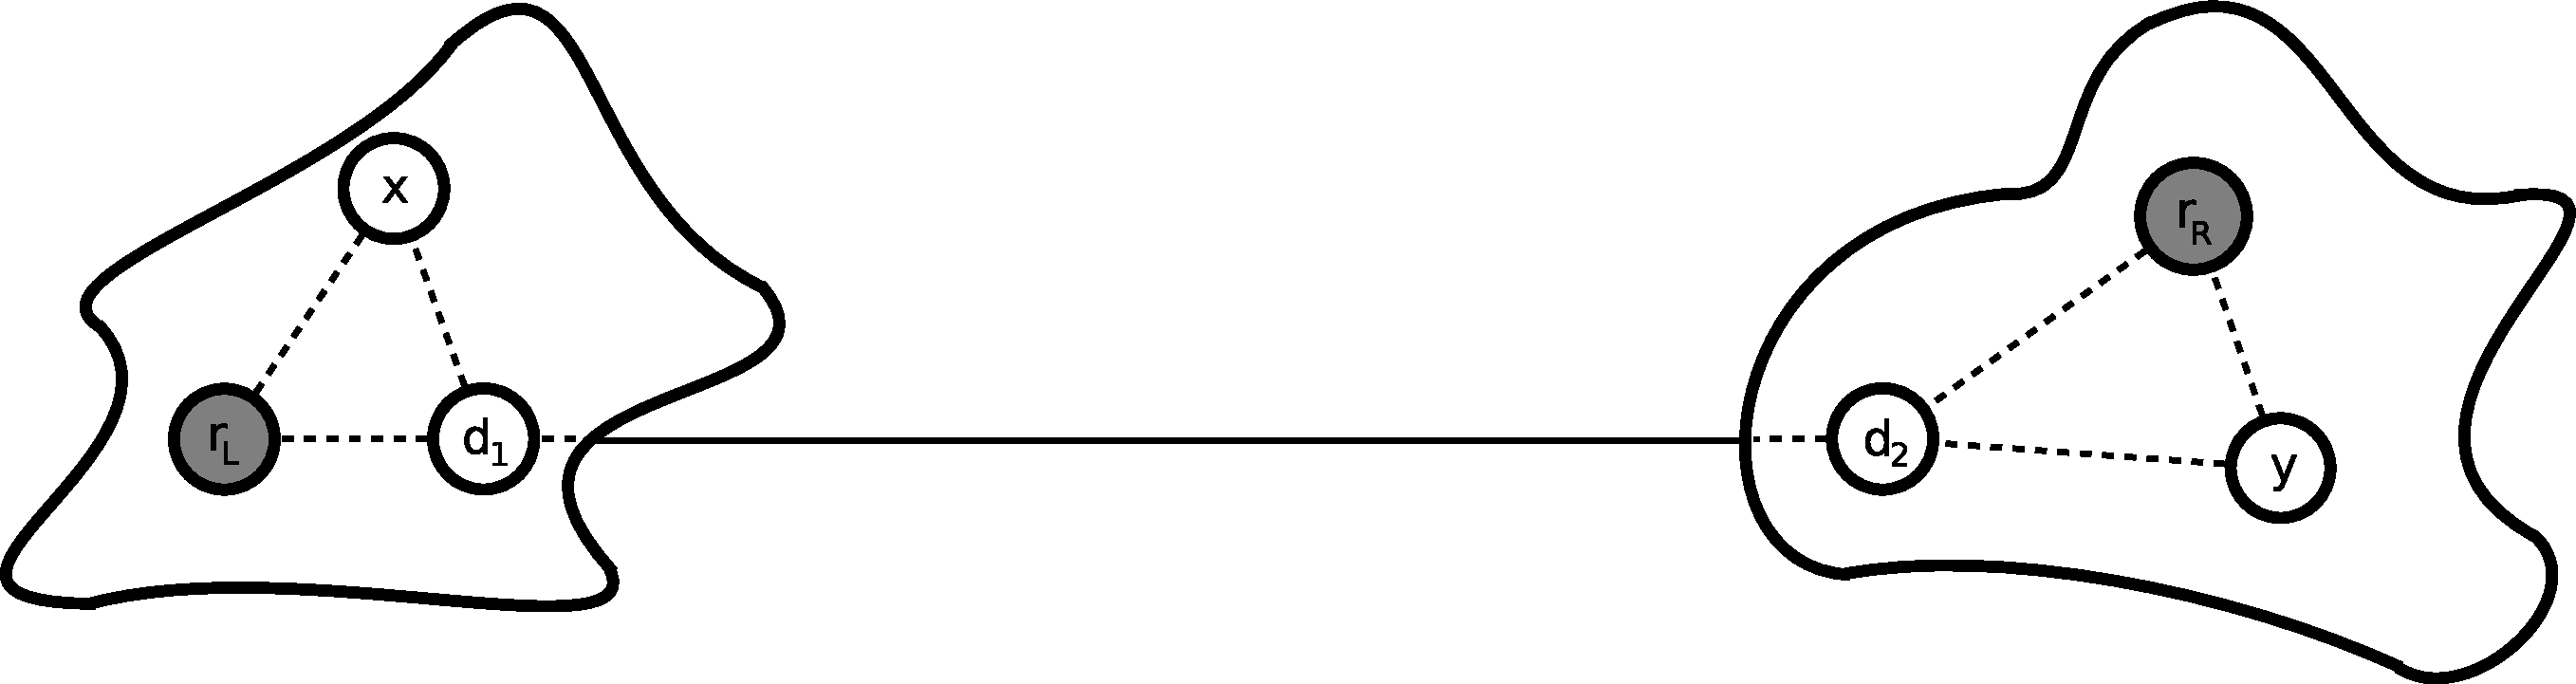
\includegraphics[width=200pt]{bilder/bew5.pdf}\newline
Alle TG mit mindestens einem Element der metrischen Basis welche durch eine Kante oder einen TG mit jeweils einem Trennungsknoten verbunden sind, haben paarweise getrennte Elemente.
}
\frame{\frametitle{Korrektheit}
\centering
\includegraphics[width=200pt]{bilder/nachbartrennungsknoten.pdf}\newline
Alle TG mit mindestens einem Element der metrischen Basis welche durch einen Trennungsnoten $v_s$, aber nicht durch eine Kante oder einen TG mit jeweils einem Trennungsknoten verbunden sind (direkt), haben paarweise getrennte Elemente oder die Nachbarschaft von $v_s$ ist nicht getrennt.

}

\frame{\frametitle{Zusammenfassung der Sätze}
Angenommen alle Komponenten sind voneinander getrennt
$\Longrightarrow$ Zu zeigen in jeder Komponente sind die Knoten getrennt. 
\begin{itemize}
\item Kreise
\item Sonnen
\item Halbsonnen
\item Bäume
\item Wege (Knoten untereinander immer getrennt, da Graph zusammenhängend und $MD\geq1$)
\end{itemize}
}
\frame{\frametitle{Zusammenfassung der Sätze}
Angenommen alle Komponenten sind untereinander getrennt
$\Longrightarrow$ Zu zeigen die direkten Nachbarschaften von Trennungsknoten sind getrennt.\\
Ist eine Komponente mit \underline{einer} einzigen Kante mit dem Trennungsknoten verbunden
\begin{itemize}
\item und beinhaltet mindestens einen Ankerknoten, so ist sie getrennt. 
\item beinhaltet keinen Ankerknoten, so ist sie ein Weg und wird als Komponente bei den AmalKnoten aufgefasst.
\end{itemize}
Sind alle Komponenten mit \underline{mehreren} Kanten mit dem Trennungsknoten verbunden $\Longrightarrow$ AmalKnoten.
}
\frame{\frametitle{Ist die Reihenfolge der Überprüfung egal?}
\begin{itemize}
\item[]
\begin{itemize}
\item[$|A|=0$] Ohne Ankerknoten gibt es keine AmalKnoten.
\item[$|A|\geq 2$] Ist die Anzahl der Ankerknoten mindestens zwei,\\so reicht ein zusätzlicher Knoten aus um, die\\Komponente untereinander und von anderen zu trennen.
\item[$|A|=1$] Für einen Ankerknoten, braucht man immer mindestens einen weiteren Knoten
\begin{itemize}
\item Sonne, Halbsonne un Kreis ungerade - man nimmt einen Knoten der die Komponenten untereinander und voneinander trennt
\item Sonne gerade - braucht man insgesamt drei Knoten
\item Halbsonne und Kreis gerade - man benötigt immer einen zusätzlichen 
\end{itemize}
\end{itemize}
\end{itemize}
}

\frame{\frametitle{Ist die Anzahl der AmalKnoten minimal?}
Es wird immer die Komponente nicht aufgenommen die nur für einen Knoten Vorteile bringt. Würde die Komponente mehr als einem Knoten Vorteile bringen, könnte man sie nicht entfernen!
}


\frame{\frametitle{Zu Beachten beim Setzen der neuen Knoten}
Ist $Weg(v)=1$ setze $MD.A$ neue Knoten.
Ist $Weg(v)=0$ setze $MD.A+1$ neue Knoten.
}


\end{document}
